\documentclass{article}
\usepackage{amsmath}
\usepackage[margin=0.5in]{geometry}
\usepackage{graphicx}
\graphicspath{ {images/} }

\setlength{\parskip}{\baselineskip}%
\setlength{\parindent}{0pt}%

\title{Homework 2}
\author{Daniel Hartig}


\begin{document}
\maketitle

\subsubsection*{1. a.)}

The Bayes classification function ($f^*$) for a piecewise function is the most likely outcome for each case. Thus for the given distribution
$$ f^* = \begin{cases} 
1,& x < 0.2, \\
-1,& 0.2 < x < 0.8,\\
1,& x > 0.8.\\ \end{cases} $$ The risk of the Bayes classification function is the probability the classification function not equalling the actual distribution of Y, or
$$ R(f^*) = \begin{cases} 
0.1,& x < 0.2, \\
0.2,& 0.2 < x < 0.8,\\
0.1,& x > 0.8.\\ \end{cases} $$
Integrating the Bayes risk function over the space ${0, 1}$ gives $0.1\cdot0.2 + 0.2\cdot0.6+0.1\cdot0.2 = 0.16$.

\subsubsection*{1. b.)}

In order for the excess risk to be zero, the classifier must have the same sign as the Bayes classification function ($f^*$) in the entire domain of $\mathcal{X}$, which is $[0, 1]$. For the specific $f^*$ given in Problem 1a, there are two changes of sign between 0 and 1. Since our function space ($\mathcal{F}$) is all polynomial functions of degree $d$, then this polynomial must have exactly two roots in the range $[0, 1]$.

For the set of all polynomial with degree $d >2$ there exists at least at least one polynomial with exactly two roots in the range $[0, 1]$. For $d=2$ and $f^*$ given above, any polynomial with roots $0.2$ and $0.8$ and no other roots in $[0, 1]$ will have excess risk equal to zero. There exists one such root $${\displaystyle (x-0.2)(x-0.8)\prod_{k = 2}^{d}(x+1)},$$ therefore $\forall f\in\mathcal{F}_d, d\geq2$; $\exists f$ such that ${\displaystyle \textrm{min}_{f\in\mathcal{F}_d} R(f) - R(f^*)}$.

For any polynomial with degree $d < 2$, there cannot be 2 roots, the classifier cannot have the same sign as $f^*$ on the domain of $\mathcal{X}$, and thus the excess risk cannot be zero. Therefore, excess risk is zero for $f\in\mathcal{F}_d$ only if $d\geq 2$.

\pagebreak
\subsubsection*{1. e.)}

Graphed images are done with 1000 iterations instead of 50 for smoother graphs. The training set is in red and independent set is in blue.

For case $d = 1$:

\begin{center}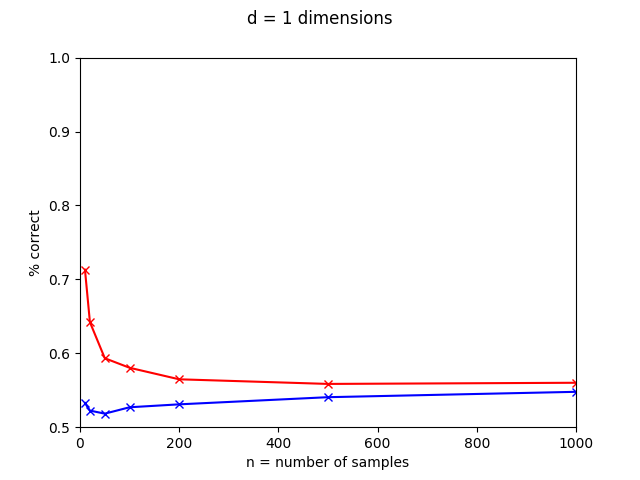
\includegraphics[scale=0.8]{dequals1}\end{center}

For case $d = 2$:

\begin{center}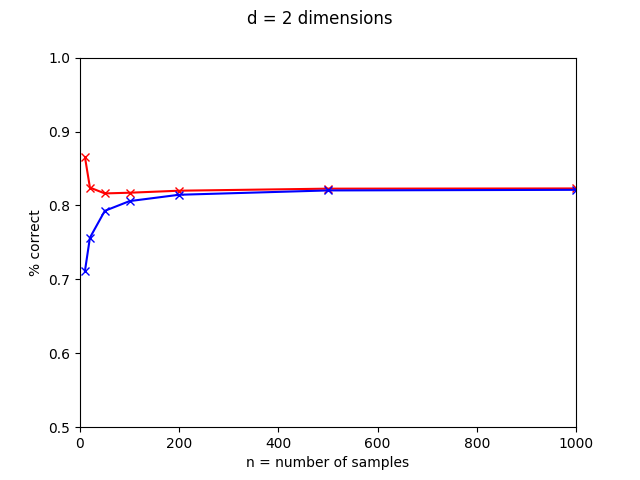
\includegraphics[scale=0.8]{dequals2}\end{center}

\pagebreak
For case $d = 5$:

\begin{center}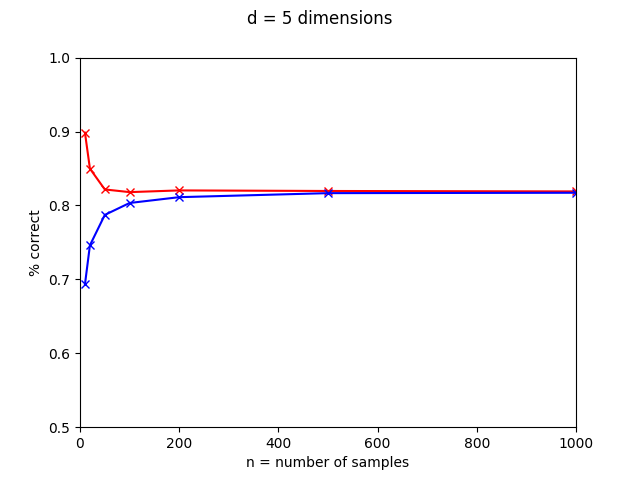
\includegraphics[scale=0.8]{dequals5}\end{center}


The disjunction between case $d=1$ and $d=2$ is  clear, as proved in section 1.b. For the first case the asymptotic correct score is $\sim0.56$ while for $ d\geq2$ score is $\sim0.82$. The asymptotic score does not quite reach the Bayes risk (which would imply score is $1-0.16=0.84$). 

For the smaller test sets, there is a relative overfitting to the training set. This means that the model fits the available data more exactly (1.e. higher than the Bayes risks says should be possible) but the actual distribution less well. As the training sample gets larger, this effect dissipates and the scores for the training set and independent set converge as the model more closely approximates the actual distribution. 

For $d=5$ the relative overfitting is more obvious than for $d=2$. The score of the n=10 training set is $\sim0.90$ for $d=5$ agaisnt $\sim0.87$ for $d=2$. This is because more variable terms allows more overfitting. 



\end{document}
